\chapter{Toxicology}

It was really the Count of Monte Cristo who had just arrived at Madame
de Villefort’s for the purpose of returning the procureur’s visit, and
at his name, as may be easily imagined, the whole house was in
confusion.

Madame de Villefort, who was alone in her drawing-room when the count
was announced, desired that her son might be brought thither instantly
to renew his thanks to the count; and Edward, who heard this great
personage talked of for two whole days, made all possible haste to come
to him, not from obedience to his mother, or out of any feeling of
gratitude to the count, but from sheer curiosity, and that some chance
remark might give him the opportunity for making one of the impertinent
speeches which made his mother say:

“Oh, that naughty child! But I can’t be severe with him, he is really
\textit{so} bright.”

After the usual civilities, the count inquired after M. de Villefort.

“My husband dines with the chancellor,” replied the young lady; “he has
just gone, and I am sure he’ll be exceedingly sorry not to have had the
pleasure of seeing you before he went.”

Two visitors who were there when the count arrived, having gazed at him
with all their eyes, retired after that reasonable delay which
politeness admits and curiosity requires.

“What is your sister Valentine doing?” inquired Madame de Villefort of
Edward; “tell someone to bid her come here, that I may have the honor
of introducing her to the count.”

“You have a daughter, then, madame?” inquired the count; “very young, I
presume?”

“The daughter of M. de Villefort by his first marriage,” replied the
young wife, “a fine well-grown girl.”

“But melancholy,” interrupted Master Edward, snatching the feathers out
of the tail of a splendid paroquet that was screaming on its gilded
perch, in order to make a plume for his hat.

Madame de Villefort merely cried, “Be still, Edward!” She then added,
“This young madcap is, however, very nearly right, and merely re-echoes
what he has heard me say with pain a hundred times; for Mademoiselle de
Villefort is, in spite of all we can do to rouse her, of a melancholy
disposition and taciturn habit, which frequently injure the effect of
her beauty. But what detains her? Go, Edward, and see.”

“Because they are looking for her where she is not to be found.”

“And where are they looking for her?”

“With grandpapa Noirtier.”

“And do you think she is not there?”

“No, no, no, no, no, she is not there,” replied Edward, singing his
words.

“And where is she, then? If you know, why don’t you tell?”

“She is under the big chestnut-tree,” replied the spoiled brat, as he
gave, in spite of his mother’s commands, live flies to the parrot,
which seemed keenly to relish such fare.

Madame de Villefort stretched out her hand to ring, intending to direct
her waiting-maid to the spot where she would find Valentine, when the
young lady herself entered the apartment. She appeared much dejected;
and any person who considered her attentively might have observed the
traces of recent tears in her eyes.

Valentine, whom we have in the rapid march of our narrative presented
to our readers without formally introducing her, was a tall and
graceful girl of nineteen, with bright chestnut hair, deep blue eyes,
and that reposeful air of quiet distinction which characterized her
mother. Her white and slender fingers, her pearly neck, her cheeks
tinted with varying hues reminded one of the lovely Englishwomen who
have been so poetically compared in their manner to the gracefulness of
a swan.

She entered the apartment, and seeing near her stepmother the stranger
of whom she had already heard so much, saluted him without any girlish
awkwardness, or even lowering her eyes, and with an elegance that
redoubled the count’s attention.

He rose to return the salutation.

“Mademoiselle de Villefort, my step-daughter,” said Madame de Villefort
to Monte Cristo, leaning back on her sofa and motioning towards
Valentine with her hand.

“And M. de Monte Cristo, King of China, Emperor of Cochin-China,” said
the young imp, looking slyly towards his sister.

Madame de Villefort at this really did turn pale, and was very nearly
angry with this household plague, who answered to the name of Edward;
but the count, on the contrary, smiled, and appeared to look at the boy
complacently, which caused the maternal heart to bound again with joy
and enthusiasm.

“But, madame,” replied the count, continuing the conversation, and
looking by turns at Madame de Villefort and Valentine, “have I not
already had the honor of meeting yourself and mademoiselle before? I
could not help thinking so just now; the idea came over my mind, and as
mademoiselle entered the sight of her was an additional ray of light
thrown on a confused remembrance; excuse the remark.”

“I do not think it likely, sir; Mademoiselle de Villefort is not very
fond of society, and we very seldom go out,” said the young lady.

“Then it was not in society that I met with mademoiselle or yourself,
madame, or this charming little merry boy. Besides, the Parisian world
is entirely unknown to me, for, as I believe I told you, I have been in
Paris but very few days. No,—but, perhaps, you will permit me to call
to mind—stay!”

The Count placed his hand on his brow as if to collect his thoughts.

“No—it was somewhere—away from here—it was—I do not know—but it appears
that this recollection is connected with a lovely sky and some
religious \textit{fête}; mademoiselle was holding flowers in her hand, the
interesting boy was chasing a beautiful peacock in a garden, and you,
madame, were under the trellis of some arbor. Pray come to my aid,
madame; do not these circumstances appeal to your memory?”

“No, indeed,” replied Madame de Villefort; “and yet it appears to me,
sir, that if I had met you anywhere, the recollection of you must have
been imprinted on my memory.”

“Perhaps the count saw us in Italy,” said Valentine timidly.

“Yes, in Italy; it was in Italy most probably,” replied Monte Cristo;
“you have travelled then in Italy, mademoiselle?”

“Yes; madame and I were there two years ago. The doctors, anxious for
my lungs, had prescribed the air of Naples. We went by Bologna,
Perugia, and Rome.”

“Ah, yes—true, mademoiselle,” exclaimed Monte Cristo as if this simple
explanation was sufficient to revive the recollection he sought. “It
was at Perugia on Corpus Christi Day, in the garden of the Hôtel des
Postes, when chance brought us together; you, Madame de Villefort, and
her son; I now remember having had the honor of meeting you.”

“I perfectly well remember Perugia, sir, and the Hôtel des Postes, and
the festival of which you speak,” said Madame de Villefort, “but in
vain do I tax my memory, of whose treachery I am ashamed, for I really
do not recall to mind that I ever had the pleasure of seeing you
before.”

“It is strange, but neither do I recollect meeting with you,” observed
Valentine, raising her beautiful eyes to the count.

\begin{figure}[ht]
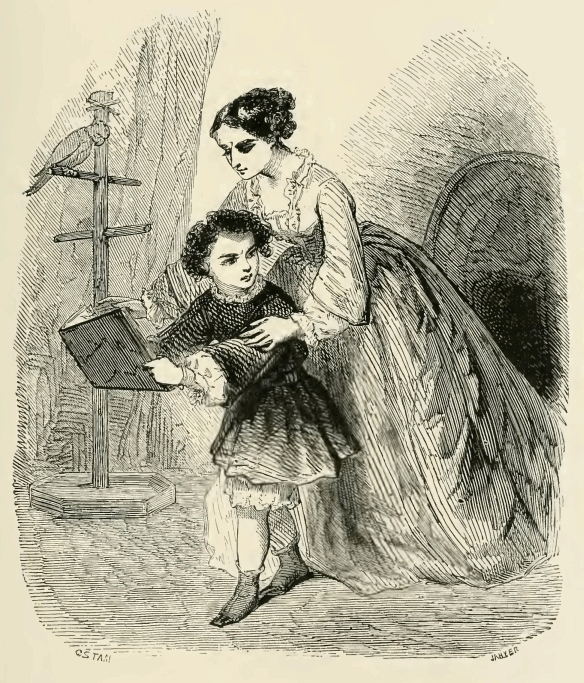
\includegraphics[width=\textwidth]{30065m.jpg}
\end{figure}

“But I remember it perfectly,” interposed the darling Edward.

“I will assist your memory, madame,” continued the count; “the day had
been burning hot; you were waiting for horses, which were delayed in
consequence of the festival. Mademoiselle was walking in the shade of
the garden, and your son disappeared in pursuit of the peacock.”

“And I caught it, mamma, don’t you remember?” interposed Edward, “and I
pulled three such beautiful feathers out of his tail.”

“You, madame, remained under the arbor; do you not remember, that while
you were seated on a stone bench, and while, as I told you,
Mademoiselle de Villefort and your young son were absent, you conversed
for a considerable time with somebody?”

“Yes, in truth, yes,” answered the young lady, turning very red, “I do
remember conversing with a person wrapped in a long woollen mantle; he
was a medical man, I think.”

“Precisely so, madame; this man was myself; for a fortnight I had been
at that hotel, during which period I had cured my valet de chambre of a
fever, and my landlord of the jaundice, so that I really acquired a
reputation as a skilful physician. We discoursed a long time, madame,
on different subjects; of Perugino, of Raphael, of manners, customs, of
the famous \textit{aqua Tofana}, of which they had told you, I think you said,
that certain individuals in Perugia had preserved the secret.”

“Yes, true,” replied Madame de Villefort, somewhat uneasily, “I
remember now.”

“I do not recollect now all the various subjects of which we
discoursed, madame,” continued the count with perfect calmness; “but I
perfectly remember that, falling into the error which others had
entertained respecting me, you consulted me as to the health of
Mademoiselle de Villefort.”

“Yes, really, sir, you were in fact a medical man,” said Madame de
Villefort, “since you had cured the sick.”

“Molière or Beaumarchais would reply to you, madame, that it was
precisely because I was not, that I had cured my patients; for myself,
I am content to say to you that I have studied chemistry and the
natural sciences somewhat deeply, but still only as an amateur, you
understand.”

At this moment the clock struck six.

“It is six o’clock,” said Madame de Villefort, evidently agitated.
“Valentine, will you not go and see if your grandpapa will have his
dinner?”

Valentine rose, and saluting the count, left the apartment without
speaking.

“Oh, madame,” said the count, when Valentine had left the room, “was it
on my account that you sent Mademoiselle de Villefort away?”

“By no means,” replied the young lady quickly; “but this is the hour
when we usually give M. Noirtier the unwelcome meal that sustains his
pitiful existence. You are aware, sir, of the deplorable condition of
my husband’s father?”

“Yes, madame, M. de Villefort spoke of it to me—a paralysis, I think.”

“Alas, yes; the poor old gentleman is entirely helpless; the mind alone
is still active in this human machine, and that is faint and
flickering, like the light of a lamp about to expire. But excuse me,
sir, for talking of our domestic misfortunes; I interrupted you at the
moment when you were telling me that you were a skilful chemist.”

“No, madame, I did not say as much as that,” replied the count with a
smile; “quite the contrary. I have studied chemistry because, having
determined to live in eastern climates I have been desirous of
following the example of King Mithridates.”

“\textit{Mithridates, rex Ponticus},” said the young scamp, as he tore some
beautiful portraits out of a splendid album, “the individual who took
cream in his cup of poison every morning at breakfast.”

“Edward, you naughty boy,” exclaimed Madame de Villefort, snatching the
mutilated book from the urchin’s grasp, “you are positively past
bearing; you really disturb the conversation; go, leave us, and join
your sister Valentine in dear grandpapa Noirtier’s room.”

“The album,” said Edward sulkily.

“What do you mean?—the album!”

“I want the album.”

“How dare you tear out the drawings?”

“Oh, it amuses me.”

“Go—go at once.”

“I won’t go unless you give me the album,” said the boy, seating
himself doggedly in an armchair, according to his habit of never giving
way.

“Take it, then, and pray disturb us no longer,” said Madame de
Villefort, giving the album to Edward, who then went towards the door,
led by his mother. The count followed her with his eyes.

“Let us see if she shuts the door after him,” he muttered.

Madame de Villefort closed the door carefully after the child, the
count appearing not to notice her; then casting a scrutinizing glance
around the chamber, the young wife returned to her chair, in which she
seated herself.

“Allow me to observe, madame,” said the count, with that kind tone he
could assume so well, “you are really very severe with that dear clever
child.”

“Oh, sometimes severity is quite necessary,” replied Madame de
Villefort, with all a mother’s real firmness.

“It was his Cornelius Nepos that Master Edward was repeating when he
referred to King Mithridates,” continued the count, “and you
interrupted him in a quotation which proves that his tutor has by no
means neglected him, for your son is really advanced for his years.”

“The fact is, count,” answered the mother, agreeably flattered, “he has
great aptitude, and learns all that is set before him. He has but one
fault, he is somewhat wilful; but really, on referring for the moment
to what he said, do you truly believe that Mithridates used these
precautions, and that these precautions were efficacious?”

“I think so, madame, because I myself have made use of them, that I
might not be poisoned at Naples, at Palermo, and at Smyrna—that is to
say, on three several occasions when, but for these precautions, I must
have lost my life.”

“And your precautions were successful?”

“Completely so.”

“Yes, I remember now your mentioning to me at Perugia something of this
sort.”

“Indeed?” said the count with an air of surprise, remarkably well
counterfeited; “I really did not remember.”

“I inquired of you if poisons acted equally, and with the same effect,
on men of the North as on men of the South; and you answered me that
the cold and sluggish habits of the North did not present the same
aptitude as the rich and energetic temperaments of the natives of the
South.”

“And that is the case,” observed Monte Cristo. “I have seen Russians
devour, without being visibly inconvenienced, vegetable substances
which would infallibly have killed a Neapolitan or an Arab.”

“And you really believe the result would be still more sure with us
than in the East, and in the midst of our fogs and rains a man would
habituate himself more easily than in a warm latitude to this
progressive absorption of poison?”

“Certainly; it being at the same time perfectly understood that he
should have been duly fortified against the poison to which he had not
been accustomed.”

“Yes, I understand that; and how would you habituate yourself, for
instance, or rather, how did you habituate yourself to it?”

“Oh, very easily. Suppose you knew beforehand the poison that would be
made use of against you; suppose the poison was, for instance,
brucine——”

“Brucine is extracted from the false angostura\footnote[8]{Brucea ferruginea.}
is it not?” inquired Madame de Villefort.

“Precisely, madame,” replied Monte Cristo; “but I perceive I have not
much to teach you. Allow me to compliment you on your knowledge; such
learning is very rare among ladies.”

“Oh, I am aware of that,” said Madame de Villefort; “but I have a
passion for the occult sciences, which speak to the imagination like
poetry, and are reducible to figures, like an algebraic equation; but
go on, I beg of you; what you say interests me to the greatest degree.”

\begin{figure}[ht]
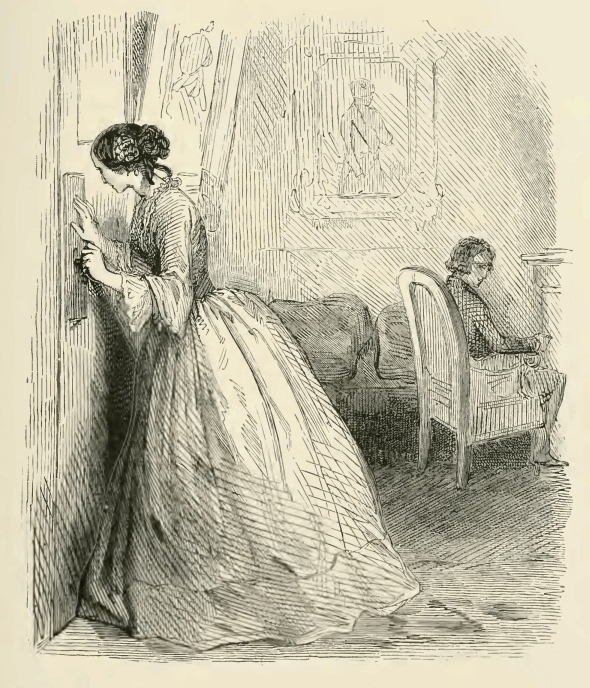
\includegraphics[width=\textwidth]{30069m.jpg}
\end{figure}

“Well,” replied Monte Cristo “suppose, then, that this poison was
brucine, and you were to take a milligramme the first day, two
milligrammes the second day, and so on. Well, at the end of ten days
you would have taken a centigramme, at the end of twenty days,
increasing another milligramme, you would have taken three hundred
centigrammes; that is to say, a dose which you would support without
inconvenience, and which would be very dangerous for any other person
who had not taken the same precautions as yourself. Well, then, at the
end of a month, when drinking water from the same carafe, you would
kill the person who drank with you, without your perceiving, otherwise
than from slight inconvenience, that there was any poisonous substance
mingled with this water.”

“Do you know any other counter-poisons?”

“I do not.”

“I have often read, and read again, the history of Mithridates,” said
Madame de Villefort in a tone of reflection, “and had always considered
it a fable.”

“No, madame, contrary to most history, it is true; but what you tell
me, madame, what you inquire of me, is not the result of a chance
query, for two years ago you asked me the same questions, and said
then, that for a very long time this history of Mithridates had
occupied your mind.”

“True, sir. The two favorite studies of my youth were botany and
mineralogy, and subsequently, when I learned that the use of simples
frequently explained the whole history of a people, and the entire life
of individuals in the East, as flowers betoken and symbolize a love
affair, I have regretted that I was not a man, that I might have been a
Flamel, a Fontana, or a Cabanis.”

“And the more, madame,” said Monte Cristo, “as the Orientals do not
confine themselves, as did Mithridates, to make a cuirass of his
poisons, but they also made them a dagger. Science becomes, in their
hands, not only a defensive weapon, but still more frequently an
offensive one; the one serves against all their physical sufferings,
the other against all their enemies. With opium, belladonna, brucea,
snake-wood, and the cherry-laurel, they put to sleep all who stand in
their way. There is not one of those women, Egyptian, Turkish, or
Greek, whom here you call ‘good women,’ who do not know how, by means
of chemistry, to stupefy a doctor, and in psychology to amaze a
confessor.”

“Really,” said Madame de Villefort, whose eyes sparkled with strange
fire at this conversation.

“Oh, yes, indeed, madame,” continued Monte Cristo, “the secret dramas
of the East begin with a love philtre and end with a death potion—begin
with paradise and end with—hell. There are as many elixirs of every
kind as there are caprices and peculiarities in the physical and moral
nature of humanity; and I will say further—the art of these chemists is
capable with the utmost precision to accommodate and proportion the
remedy and the bane to yearnings for love or desires for vengeance.”

“But, sir,” remarked the young woman, “these Eastern societies, in the
midst of which you have passed a portion of your existence, are as
fantastic as the tales that come from their strange land. A man can
easily be put out of the way there, then; it is, indeed, the Bagdad and
Bassora of the \textit{Thousand and One Nights}. The sultans and viziers who
rule over society there, and who constitute what in France we call the
government, are really Haroun-al-Raschids and Giaffars, who not only
pardon a poisoner, but even make him a prime minister, if his crime has
been an ingenious one, and who, under such circumstances, have the
whole story written in letters of gold, to divert their hours of
idleness and \textit{ennui}.”

“By no means, madame; the fanciful exists no longer in the East. There,
disguised under other names, and concealed under other costumes, are
police agents, magistrates, attorneys-general, and bailiffs. They hang,
behead, and impale their criminals in the most agreeable possible
manner; but some of these, like clever rogues, have contrived to escape
human justice, and succeed in their fraudulent enterprises by cunning
stratagems. Amongst us a simpleton, possessed by the demon of hate or
cupidity, who has an enemy to destroy, or some near relation to dispose
of, goes straight to the grocer’s or druggist’s, gives a false name,
which leads more easily to his detection than his real one, and under
the pretext that the rats prevent him from sleeping, purchases five or
six grammes of arsenic—if he is really a cunning fellow, he goes to
five or six different druggists or grocers, and thereby becomes only
five or six times more easily traced;—then, when he has acquired his
specific, he administers duly to his enemy, or near kinsman, a dose of
arsenic which would make a mammoth or mastodon burst, and which,
without rhyme or reason, makes his victim utter groans which alarm the
entire neighborhood. Then arrive a crowd of policemen and constables.
They fetch a doctor, who opens the dead body, and collects from the
entrails and stomach a quantity of arsenic in a spoon. Next day a
hundred newspapers relate the fact, with the names of the victim and
the murderer. The same evening the grocer or grocers, druggist or
druggists, come and say, ‘It was I who sold the arsenic to the
gentleman;’ and rather than not recognize the guilty purchaser, they
will recognize twenty. Then the foolish criminal is taken, imprisoned,
interrogated, confronted, confounded, condemned, and cut off by hemp or
steel; or if she be a woman of any consideration, they lock her up for
life. This is the way in which you Northerns understand chemistry,
madame. Desrues was, however, I must confess, more skilful.”

“What would you have, sir?” said the lady, laughing; “we do what we
can. All the world has not the secret of the Medicis or the Borgias.”

“Now,” replied the count, shrugging his shoulders, “shall I tell you
the cause of all these stupidities? It is because, at your theatres, by
what at least I could judge by reading the pieces they play, they see
persons swallow the contents of a phial, or suck the button of a ring,
and fall dead instantly. Five minutes afterwards the curtain falls, and
the spectators depart. They are ignorant of the consequences of the
murder; they see neither the police commissary with his badge of
office, nor the corporal with his four men; and so the poor fools
believe that the whole thing is as easy as lying. But go a little way
from France—go either to Aleppo or Cairo, or only to Naples or Rome,
and you will see people passing by you in the streets—people erect,
smiling, and fresh-colored, of whom Asmodeus, if you were holding on by
the skirt of his mantle, would say, ‘That man was poisoned three weeks
ago; he will be a dead man in a month.’”

“Then,” remarked Madame de Villefort, “they have again discovered the
secret of the famous \textit{aqua Tofana} that they said was lost at Perugia.”

“Ah, but madame, does mankind ever lose anything? The arts change about
and make a tour of the world; things take a different name, and the
vulgar do not follow them—that is all; but there is always the same
result. Poisons act particularly on some organ or another—one on the
stomach, another on the brain, another on the intestines. Well, the
poison brings on a cough, the cough an inflammation of the lungs, or
some other complaint catalogued in the book of science, which, however,
by no means precludes it from being decidedly mortal; and if it were
not, would be sure to become so, thanks to the remedies applied by
foolish doctors, who are generally bad chemists, and which will act in
favor of or against the malady, as you please; and then there is a
human being killed according to all the rules of art and skill, and of
whom justice learns nothing, as was said by a terrible chemist of my
acquaintance, the worthy Abbé Adelmonte of Taormina, in Sicily, who has
studied these national phenomena very profoundly.”

“It is quite frightful, but deeply interesting,” said the young lady,
motionless with attention. “I thought, I must confess, that these
tales, were inventions of the Middle Ages.”

“Yes, no doubt, but improved upon by ours. What is the use of time,
rewards of merit, medals, crosses, Monthyon prizes, if they do not lead
society towards more complete perfection? Yet man will never be perfect
until he learns to create and destroy; he does know how to destroy, and
that is half the battle.”

“So,” added Madame de Villefort, constantly returning to her object,
“the poisons of the Borgias, the Medicis, the Renées, the Ruggieris,
and later, probably, that of Baron de Trenck, whose story has been so
misused by modern drama and romance——”

“Were objects of art, madame, and nothing more,” replied the count. “Do
you suppose that the real \textit{savant} addresses himself stupidly to the
mere individual? By no means. Science loves eccentricities, leaps and
bounds, trials of strength, fancies, if I may be allowed so to term
them. Thus, for instance, the excellent Abbé Adelmonte, of whom I spoke
just now, made in this way some marvellous experiments.”

“Really?”

“Yes; I will mention one to you. He had a remarkably fine garden, full
of vegetables, flowers, and fruit. From amongst these vegetables he
selected the most simple—a cabbage, for instance. For three days he
watered this cabbage with a distillation of arsenic; on the third, the
cabbage began to droop and turn yellow. At that moment he cut it. In
the eyes of everybody it seemed fit for table, and preserved its
wholesome appearance. It was only poisoned to the Abbé Adelmonte. He
then took the cabbage to the room where he had rabbits—for the Abbé
Adelmonte had a collection of rabbits, cats, and guinea-pigs, fully as
fine as his collection of vegetables, flowers, and fruit. Well, the
Abbé Adelmonte took a rabbit, and made it eat a leaf of the cabbage.
The rabbit died. What magistrate would find, or even venture to
insinuate, anything against this? What procureur has ever ventured to
draw up an accusation against M. Magendie or M. Flourens, in
consequence of the rabbits, cats, and guinea-pigs they have killed?—not
one. So, then, the rabbit dies, and justice takes no notice. This
rabbit dead, the Abbé Adelmonte has its entrails taken out by his cook
and thrown on the dunghill; on this dunghill is a hen, who, pecking
these intestines, is in her turn taken ill, and dies next day. At the
moment when she is struggling in the convulsions of death, a vulture is
flying by (there are a good many vultures in Adelmonte’s country); this
bird darts on the dead fowl, and carries it away to a rock, where it
dines off its prey. Three days afterwards, this poor vulture, which has
been very much indisposed since that dinner, suddenly feels very giddy
while flying aloft in the clouds, and falls heavily into a fish-pond.
The pike, eels, and carp eat greedily always, as everybody knows—well,
they feast on the vulture. Now suppose that next day, one of these
eels, or pike, or carp, poisoned at the fourth remove, is served up at
your table. Well, then, your guest will be poisoned at the fifth
remove, and die, at the end of eight or ten days, of pains in the
intestines, sickness, or abscess of the pylorus. The doctors open the
body and say with an air of profound learning, ‘The subject has died of
a tumor on the liver, or of typhoid fever!’”

“But,” remarked Madame de Villefort, “all these circumstances which you
link thus to one another may be broken by the least accident; the
vulture may not see the fowl, or may fall a hundred yards from the
fish-pond.”

“Ah, that is where the art comes in. To be a great chemist in the East,
one must direct chance; and this is to be achieved.”

Madame de Villefort was in deep thought, yet listened attentively.

“But,” she exclaimed, suddenly, “arsenic is indelible, indestructible;
in whatsoever way it is absorbed, it will be found again in the body of
the victim from the moment when it has been taken in sufficient
quantity to cause death.”

“Precisely so,” cried Monte Cristo—“precisely so; and this is what I
said to my worthy Adelmonte. He reflected, smiled, and replied to me by
a Sicilian proverb, which I believe is also a French proverb, ‘My son,
the world was not made in a day—but in seven. Return on Sunday.’ On the
Sunday following I did return to him. Instead of having watered his
cabbage with arsenic, he had watered it this time with a solution of
salts, having their basis in strychnine, \textit{strychnos colubrina}, as the
learned term it. Now, the cabbage had not the slightest appearance of
disease in the world, and the rabbit had not the smallest distrust;
yet, five minutes afterwards, the rabbit was dead. The fowl pecked at
the rabbit, and the next day was a dead hen. This time we were the
vultures; so we opened the bird, and this time all special symptoms had
disappeared, there were only general symptoms. There was no peculiar
indication in any organ—an excitement of the nervous system—that was
it; a case of cerebral congestion—nothing more. The fowl had not been
poisoned—she had died of apoplexy. Apoplexy is a rare disease among
fowls, I believe, but very common among men.”

Madame de Villefort appeared more and more thoughtful.

“It is very fortunate,” she observed, “that such substances could only
be prepared by chemists; otherwise, all the world would be poisoning
each other.”

“By chemists and persons who have a taste for chemistry,” said Monte
Cristo carelessly.

“And then,” said Madame de Villefort, endeavoring by a struggle, and
with effort, to get away from her thoughts, “however skilfully it is
prepared, crime is always crime, and if it avoid human scrutiny, it
does not escape the eye of God. The Orientals are stronger than we are
in cases of conscience, and, very prudently, have no hell—that is the
point.”

\begin{figure}[ht]
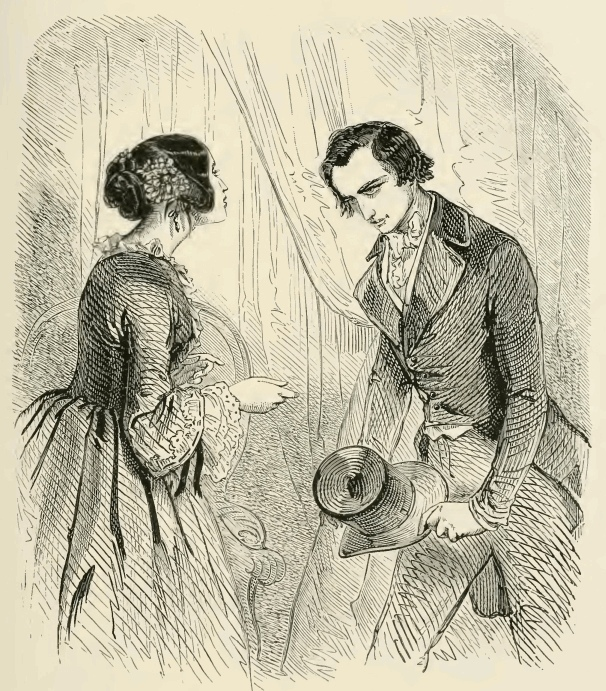
\includegraphics[width=\textwidth]{30075m.jpg}
\end{figure}

“Really, madame, this is a scruple which naturally must occur to a pure
mind like yours, but which would easily yield before sound reasoning.
The bad side of human thought will always be defined by the paradox of
Jean Jacques Rousseau,—you remember,—the mandarin who is killed five
hundred leagues off by raising the tip of the finger. Man’s whole life
passes in doing these things, and his intellect is exhausted by
reflecting on them. You will find very few persons who will go and
brutally thrust a knife in the heart of a fellow-creature, or will
administer to him, in order to remove him from the surface of the globe
on which we move with life and animation, that quantity of arsenic of
which we just now talked. Such a thing is really out of rule—eccentric
or stupid. To attain such a point, the blood must be heated to
thirty-six degrees, the pulse be, at least, at ninety, and the feelings
excited beyond the ordinary limit. But suppose one pass, as is
permissible in philology, from the word itself to its softened synonym,
then, instead of committing an ignoble assassination you make an
‘elimination;’ you merely and simply remove from your path the
individual who is in your way, and that without shock or violence,
without the display of the sufferings which, in the case of becoming a
punishment, make a martyr of the victim, and a butcher, in every sense
of the word, of him who inflicts them. Then there will be no blood, no
groans, no convulsions, and above all, no consciousness of that horrid
and compromising moment of accomplishing the act,—then one escapes the
clutch of the human law, which says, ‘Do not disturb society!’ This is
the mode in which they manage these things, and succeed in Eastern
climes, where there are grave and phlegmatic persons who care very
little for the questions of time in conjunctures of importance.”

“Yet conscience remains,” remarked Madame de Villefort in an agitated
voice, and with a stifled sigh.

“Yes,” answered Monte Cristo “happily, yes, conscience does remain; and
if it did not, how wretched we should be! After every action requiring
exertion, it is conscience that saves us, for it supplies us with a
thousand good excuses, of which we alone are judges; and these reasons,
howsoever excellent in producing sleep, would avail us but very little
before a tribunal, when we were tried for our lives. Thus Richard III.,
for instance, was marvellously served by his conscience after the
putting away of the two children of Edward IV.; in fact, he could say,
‘These two children of a cruel and persecuting king, who have inherited
the vices of their father, which I alone could perceive in their
juvenile propensities—these two children are impediments in my way of
promoting the happiness of the English people, whose unhappiness they
(the children) would infallibly have caused.’ Thus was Lady Macbeth
served by her conscience, when she sought to give her son, and not her
husband (whatever Shakespeare may say), a throne. Ah, maternal love is
a great virtue, a powerful motive—so powerful that it excuses a
multitude of things, even if, after Duncan’s death, Lady Macbeth had
been at all pricked by her conscience.”

Madame de Villefort listened with avidity to these appalling maxims and
horrible paradoxes, delivered by the count with that ironical
simplicity which was peculiar to him.

After a moment’s silence, the lady inquired:

“Do you know, my dear count,” she said, “that you are a very terrible
reasoner, and that you look at the world through a somewhat distempered
medium? Have you really measured the world by scrutinies, or through
alembics and crucibles? For you must indeed be a great chemist, and the
elixir you administered to my son, which recalled him to life almost
instantaneously——”

\begin{figure}[ht]
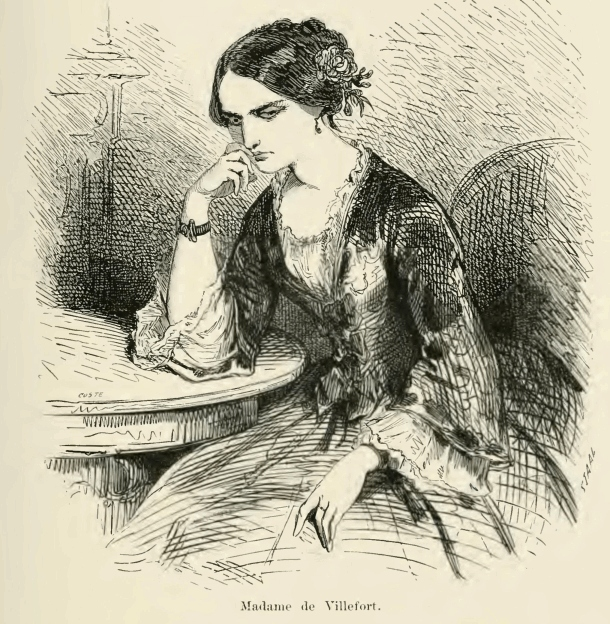
\includegraphics[width=\textwidth]{30077m.jpg}
\end{figure}

“Oh, do not place any reliance on that, madame; \textit{one} drop of that
elixir sufficed to recall life to a dying child, but three drops would
have impelled the blood into his lungs in such a way as to have
produced most violent palpitations; six would have suspended his
respiration, and caused syncope more serious than that in which he was;
ten would have destroyed him. You know, madame, how suddenly I snatched
him from those phials which he so imprudently touched?”

“Is it then so terrible a poison?”

“Oh, no! In the first place, let us agree that the word poison does not
exist, because in medicine use is made of the most violent poisons,
which become, according as they are employed, most salutary remedies.”

“What, then, is it?”

“A skilful preparation of my friend’s the worthy Abbé Adelmonte, who
taught me the use of it.”

“Oh,” observed Madame de Villefort, “it must be an admirable
anti-spasmodic.”

“Perfect, madame, as you have seen,” replied the count; “and I
frequently make use of it—with all possible prudence though, be it
observed,” he added with a smile of intelligence.

“Most assuredly,” responded Madame de Villefort in the same tone. “As
for me, so nervous, and so subject to fainting fits, I should require a
Doctor Adelmonte to invent for me some means of breathing freely and
tranquillizing my mind, in the fear I have of dying some fine day of
suffocation. In the meanwhile, as the thing is difficult to find in
France, and your abbé is not probably disposed to make a journey to
Paris on my account, I must continue to use Monsieur Planche’s
anti-spasmodics; and mint and Hoffman’s drops are among my favorite
remedies. Here are some lozenges which I have made up on purpose; they
are compounded doubly strong.”

Monte Cristo opened the tortoise-shell box, which the lady presented to
him, and inhaled the odor of the lozenges with the air of an amateur
who thoroughly appreciated their composition.

“They are indeed exquisite,” he said; “but as they are necessarily
submitted to the process of deglutition—a function which it is
frequently impossible for a fainting person to accomplish—I prefer my
own specific.”

“Undoubtedly, and so should I prefer it, after the effects I have seen
produced; but of course it is a secret, and I am not so indiscreet as
to ask it of you.”

“But I,” said Monte Cristo, rising as he spoke—“I am gallant enough to
offer it you.”

\begin{figure}[ht]
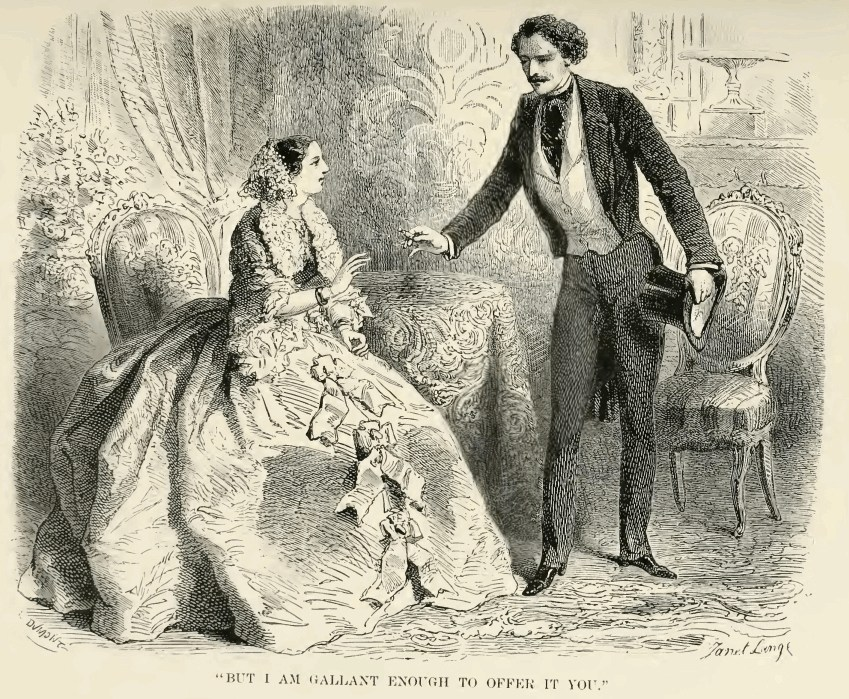
\includegraphics[width=\textwidth]{30079m.jpg}
\end{figure}

“How kind you are.”

“Only remember one thing—a small dose is a remedy, a large one is
poison. One drop will restore life, as you have seen; five or six will
inevitably kill, and in a way the more terrible inasmuch as, poured
into a glass of wine, it would not in the slightest degree affect its
flavor. But I say no more, madame; it is really as if I were
prescribing for you.”

The clock struck half-past six, and a lady was announced, a friend of
Madame de Villefort, who came to dine with her.

“If I had had the honor of seeing you for the third or fourth time,
count, instead of only for the second,” said Madame de Villefort; “if I
had had the honor of being your friend, instead of only having the
happiness of being under an obligation to you, I should insist on
detaining you to dinner, and not allow myself to be daunted by a first
refusal.”

“A thousand thanks, madame,” replied Monte Cristo “but I have an
engagement which I cannot break. I have promised to escort to the
Académie a Greek princess of my acquaintance who has never seen your
grand opera, and who relies on me to conduct her thither.”

“Adieu, then, sir, and do not forget the prescription.”

“Ah, in truth, madame, to do that I must forget the hour’s conversation
I have had with you, which is indeed impossible.”

Monte Cristo bowed, and left the house. Madame de Villefort remained
immersed in thought.

“He is a very strange man,” she said, “and in my opinion is himself the
Adelmonte he talks about.”

As to Monte Cristo the result had surpassed his utmost expectations.

“Good,” said he, as he went away; “this is a fruitful soil, and I feel
certain that the seed sown will not be cast on barren ground.”

Next morning, faithful to his promise, he sent the prescription
requested.
